\documentclass{SeminarV2}

\usepackage[latin1]{inputenc}
\usepackage{amssymb,amsmath,array}
\usepackage{graphicx}
\usepackage{placeins}

\usepackage{fancyvrb}
\fvset{tabsize=4}

\usepackage{hyperref}
\usepackage{framed}


\usepackage{listings}

\lstset{%
	language=[LaTeX]TeX,
	basicstyle=\ttfamily,
	breaklines=true,
	columns=fullflexible
}

\newcommand{\shellcmd}[1]{\\\indent\indent\texttt{\footnotesize\$ #1}\\}

\newcommand{\mV}{multiVitamin }


%
\voffset 0 cm \hoffset -1 cm \addtolength{\textwidth}{2cm}
\addtolength{\textheight}{0cm}\addtolength{\leftmargin}{0cm}



\begin{document}
%style file for Seminar manuscripts
\title{User Manual}

%***********************************************************************
% AUTHORS INFORMATION AREA
%***********************************************************************
\author{Maximilian Joas$^1$, Michel Kreck�$^1$
%
% Optional short acknowledgment: remove next line if non-needed
%\thanks{This is an optional funding source acknowledgement.}
%
% DO NOT MODIFY THE FOLLOWING '\vspace' ARGUMENT
\vspace{.3cm}\\
%
% Addresses and institutions (remove "1- " in case of a single institution)
University of Leipzig  - Department of Computer Science \\
Augustusplatz 10, 04109 Leipzig  - Germany\\}

%
% Remove the next three lines in case of a single institution

%***********************************************************************
% END OF AUTHORS INFORMATION AREA
%***********************************************************************

\maketitle

\begin{abstract}


\end{abstract}

\section{multiVitamin}
\mV is a software package which allows users to perform multiple alignments with graphs.
There are two algorithms available for this task. The Bron Kerbosch \cite{}
and the VF2 algorithm \cite{}. Details on the algorithms ca be found in the
theory section.\\
The main function of the package is to align two or more graphs. This results in a binary alignment guide tree containing the "best" alignment procedure. The resulting multiple graph alignment is represented as a graph itself.\cite{}  
Sounds exciting, so let's get started!

\section{Installation}

Clone the repo from github with 
\shellcmd{git clone https://github.com/mk36fyvy/multivitamin.git}
Navigate to the directory containing the setup.py file and type 
\shellcmd{pip3 install .}
%cd multivitamin_project/multivitamin/multivitamin
Done, now you can run \mV in the command shell. You can test if the installation was successful by typing
\shellcmd{multiVitamin -h}



\section{Graph Format}

A good first step is to familiarize yourself with the graph format. A graph
file is basically a text file, we use the extension .graph to be more specific. It is also used interiorly to identify graph files as such.

Every graph consists of nodes and edges. Every node has an id, which is an unique
integer (handled as a String internally most of the time) for each node. Optionally, nodes can be labelled. The id and label are separated by a semicolon (\texttt{;}). The edges are two connected nodes and represented
by the ids of the two nodes separated with a semicolon.\\

The file itself is structured as follows (see below for an \hyperref[fig:graph_example]{example}): \\

\begin{itemize}
	\item In the first paragraph, there is a possibility to insert comment lines by preceding comments with \texttt{//} or writing \texttt{;comment} after the comment. These lines will be ignored by the parser.
	\item The first line indicates the author of the graph. This line has to start with the word "author" to be recognized by the parser.
	\item The second and third lines show the number of nodes and edges respectively. The parser only sees two consecutive integers at the end of the lines, so it is important that the number of nodes is provided before the number of edges.
	\item The next three lines are booleans that indicate whether the nodes / edges are labelled and if the graph is directed. It is important to stick to the order indicated in the \hyperref[fig:graph_example]{example} below.
	\item The blank line indicates the start of the node section. It is important to choose an integer as node id. The label can be any symbol, except for \texttt{;}.
	\item The node section is separated from the edge section again by a blank line. If the \texttt{Directed graph} option is set to \texttt{False}, the edges are considered undirected. Internally, every edge's reverse is then added to the graph.  
\end{itemize}

\noindent
Let's look at a small example graph for illustration. The graph has 6 nodes
which are all labelled with a 'c' and 6 edged which are not labelled.
Your graphs need to have exactly this format to use this package. especially
the blank lines are important. For further example graphs go to the root
You can also put comments in your graph files with //.
directory and navigate to the graphs directory. Now that you are familiar with
the graph format, we can take a look how to use the package.


\begin{framed}
\label{fig:graph_example}
\begin{verbatim} 
AUTHOR: Michel K.
#nodes;6
#edges;6
Nodes labelled;True
Edges labelled;False
Directed graph;False

1;c
2;c
3;c
4;c
5;c
6;c

1;2
1;6
2;3
3;4
4;5
5;6
\end{verbatim}
\end{framed}

\section{Graph Alignment basic case}
Consider the basic use without any optional flags for the start.
You do \textbf{not} have to be in the directory of the package to use \mV.
To get an overview of all the flags you can type 
\shellcmd{multiVitamin -h}
If you have experience with command-line tools the information provided by multivitamin -h
may be sufficient to get you started.\\

\begin{lstlisting}
multiVitamin - A multiple alignment tool for graphs

optional arguments:
  -h, --help            show this help message and exit
  -a ALGORITHM, --algorithm ALGORITHM
                        choose an alignment-algorithm (BK or VF2) (default: BK)
                         Warning: VF2 is only suited if there is true graph-subgraph isomorphism!
  -s, --save-all        save all the graphs produced during the alignment
                         The graphs are saved as "[newick].graph"
  -t, --save-shorter    save an additional version of the alignment graph with much shorter node ids
  -g, --save-guide      save the guide tree in Newick-format as "tree.txt"

required arguments:
  these arguments are mutually exclusive

  -m FILES [FILES ...]  provide .graph files for multiple alignment. '.' is a valid input
  -c COOPT [COOPT ...]  provide *2* graphs which will be aligned. Co-optimals will be saved in ./results.
  -v VIEW               get a visual representation of *1* given graph
\end{lstlisting}

There are three mutually exclusive flags. One of them is always
required to make multiVitamin work. For the start we look at the
case of a multiple alignment of graphs, which will be the standard use case.
The flag for that is -m. The other flags are explained later.
Just type "mulitVitamin -m <pathToGraphFile1.graph> <pathToGraphFile2> <optionalMoreGraphFiles>"
in the command line. This aligns the given graphs with the Bron Kerbosch algorithmn.
The resulting command line seems confusing at first put follows a clear structure
and provides all the important information about the alignment."
in the command line. This aligns the given graphs with the Bron Kerbosch algorithmn.
The resulting command line seems confusing at first put follows a clear structure
and provides all the important information about the alignment.
In order to see from which graph each node of the alignent origins, we use
abbrevations of the names of the graph input files. A dictionary of the abbrevations
of the original names of the graph files is shown first in the command line output.
The you see the nodes of the alignment. Each line corresponds to one node
of the alignment. A node in an alignment is represented by all nodes that got mathed
to eachother. The aligned node is represented as follows:
The id of th enode consits of the graph id (more specific of the abbrevation of the graph id) of the
graph where the node origins from. This is followed by a colon, followed by the id
of the original node. after a dot comes the next aligned node. After that
 follows a tab and the label of the aligned node (if the graphs were labelled).
After another tab the neighbors of the node are listed. The next line shows
the same for the next node of the alignment.\\
The next section shows the edges of the aligned graph. The format follows the format
of the edges. It basically shows to nodes seperated by a comma and a tab. \\
Additionally to the command line output multiVitamin creates a result folder.
This folder contains the aligned graph as .graph file. The first line of the
.graph file shows the Newik tree of the mulitple alignment.
This file could theoretically
be used for further computation with mulitVitamin. The results folder contains
also a .txt file of the abbrevations of the graph files. These abbrevations are
used to indicate in the alignment which node origins from which graph.\\
\begin{figure}
     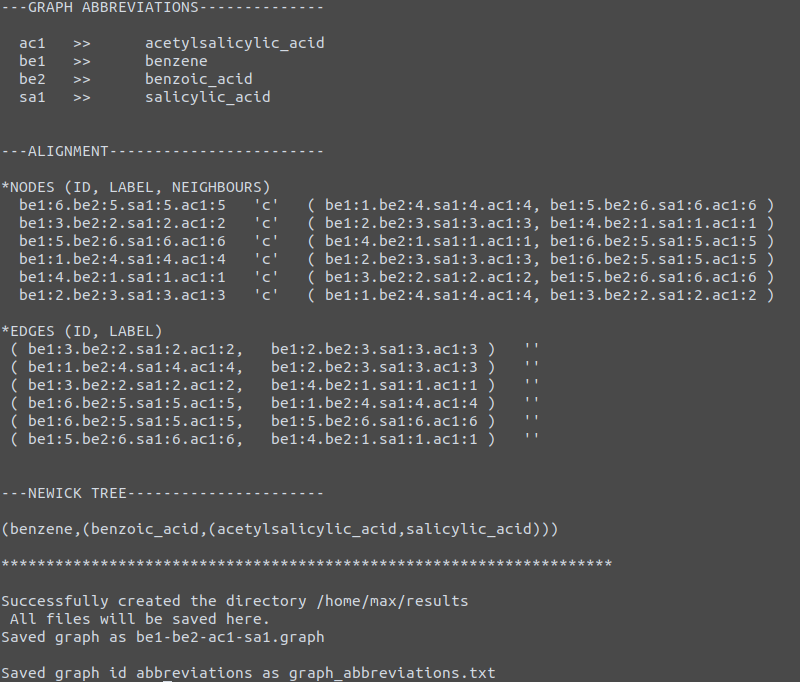
\includegraphics[width=0.5\textwidth]{multiOUT.png}
  \caption{A sample output of a multiple graph alignment}
\end{figure}


\subsection{Graph Alignment with the Vf2}
Let us still consider the basic use case with the required flag -m. This flag can
be combined with all optional flags (see section advanced use). One of those optional
flags is -a which specifies the algorithmn that will be used for the alignent.

In order to use the VF2 algorithmn for the alignent you have to use the flag
-a with  "vf2" as parameter in additon to the specification of the input files. So the command would be
"mulitVitamin -f <pathToGraphFile1.graph> <pathToGraphFile2> <optionalMoreGraphFiles>" -a vf2"
This option is only suited for subgraph graph isomorphisms. So the smaller graph
must always fit entirely in the bigger graph. Despite this restriction the
Vf2 is able to align graphs based on the label of the node ids. So a structural
isomorphism is not enough in this case, but the nodes that could aligned
structurally must also fulfill some kind of semantic condition. This is
usefull to align chemical molecules that are represented as graphs.
This condition can be determined by the user in the custom.py

\subsubsection{Custom.py}
The custom.py file can be found in the multivitamin directory of the root folder.
This file contains a functino the check\_semantics function, which by default
returns always true. The code of the custom.py file looks as follows:
\begin{verbatim}[numbers=left,xleftmargin=5mm]
def check_semantics( n, m ):
    '''This function is used in VF2 algorithm to decide,
    whether aligning to nodes is allowed from the
    label point of view.
    In the sample example below, two nodes will only
    be accepted as a legal matching, if the two
    labels are exactly the same.

    Insert your scoring logic below:'''

#    if n.label == m.label:
#        return True
#    else:
#        return False

    return True

def get_results_dir():
    '''define, where the result files will be saved.
    Default is a dir named 'results' in the current
    working directory'''

    return "/results"
\end{verbatim}

If you untoggle the single comments and out-comment the return True, you get a simple
semantic check that only allows nodes to be aligned that have the same label.
However you can go as crazy as you want with it.\\
Besides the check\_semantics method you can also specify the path where your
results should be saved. Just specify your prefered path as a string as return
value from get\_results\_dir(). Before we jump into the supplemtary clasees, which
you might want to modify for a highly sophisticated check\_semantics function, we
want to take a look at the other flag options.
Note: A change in the supplemtary classes is not recommended.
\section{Advanced Usage}
To make multiVitamin work you need one (exactely one) of the following flags:
-m, -c, -v.\\
The -m option has been discussed in depth in the previous sections. It can be used with
every optional flag.\\
The -v flag allows for graphical representation of our .graph files.
You need to proved a graph file. In most cases this will be the graph of the mulitple
alignent. Use: "multiVitamin -v <file.graph>"
It is not compatible with any of the optional flags.\\
The -c flag works only for exactely two input files.
It gives all the co-optimal alignments of the two given graphs. There exist
cases where two graphs have more can be aligned in different, yet optimal ways.
The -c flag calculates all these cases.
Since -c only works with 2 graphs the Optional flags are not helpful.
Only the -a flag could be used to use the vf2 algorithm. Note lead to high
computation costs.
Let us consider the optional flags now.
If you want to save the guide tree in an extra file use -g.
If you not only want the final multiple alignment graph, but also
all alignments in between use -s. If you have three graphs for example graph1, graph2
and graph3. Let us assume multiVitamin gives us a graph which multiple alignment
is represented by this Newick tree: ((graph1,graph2),graph3). Now you
with the option -s you will also get the alignment of graph1 and graph2 as a graph file.\\

\section{Basic Classes}
In order to implement the Bron Kerbosch and Vf2 algorithm, we used three classes.
A graph class, a node class and a edge class. In general the classes should not be altered
by the user. However for the sophisticated user there may be cases in which he or she
wants to make adjustments to this classes. Therefore we will given a brief
overview of them. Figure 2 shows simple UML diagrams of our base classes. The most important methods and attributes will be explained.
\begin{figure}
    %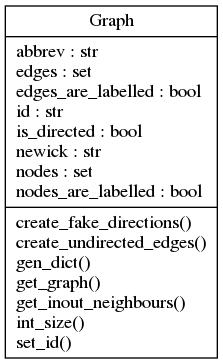
\includegraphics[width=0.5\textwidth]{classes.png}
    %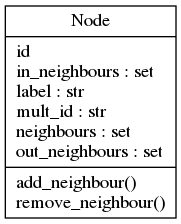
\includegraphics[width=0.5\textwidth]{node.png}
    %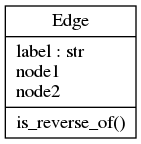
\includegraphics[width=0.5\textwidth]{edge.png}
	{\centering
	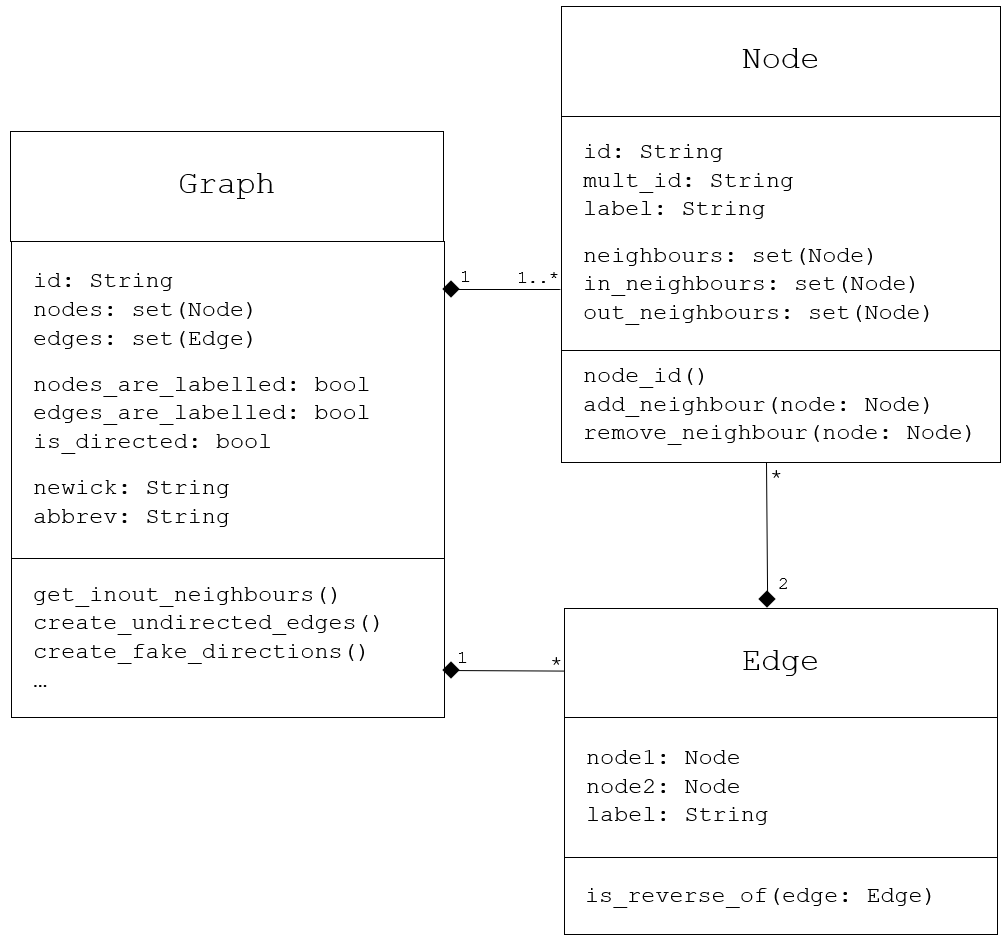
\includegraphics[scale=1.7]{multivitamin_basic_uml.png}
}

  \caption{A UML class diagram of the base classes}
\end{figure}
\subsection{Node}
Our node objects are seen in the context of a graph. Thus every node contains information about
its neighbours. Therefore a node has a neighbours attribute which is a set of Node objects.
In case of directed graphs one can distingush between in and out neighbours. Thus a node object has a seperate set for these two kind of neighbours. This is useful in the Vf2 algorithmn. The mult\_id attribute gives an option to name the node in a mulitple alignment.
\subsubsection{Edge}
An Edge consits of two node objects and an optional label. For each Edge canbe checked if it is the reverse of another edge. This only makes sense for directed graphs.
\subsection{Graph Class}
Besides the obvious attributes of nodes, edges and an id, a graph objects also as an
abbrev which is TODO. Since the Vf2 only works with directed graphs, we 
gave our graphs the possibility to give the graph directions. Consider the Edge A-B. The 
create\_fake\_directions method now points node A to B and node B to A.\\
The method create\_undirected\_edges fills the edge set of the Graph with help of the neighbour set of the node class. The method get\_inout\_neighbours fills the in and outneighbour sets of the node objects in the node set.\\\\
All classes have build in print mehtods for more readable output as well as build in 
methods to compare the objects. So you can determine which graph is larger by the amount of 
nodes in the nodes sets and also determine if two graphs are equal based on their id.\\
Nodes can be also compared by its id and edges by the ids of their nodes.
\section{Theoretical Foundations of the Algorithmns}

\subsection{Bron Kerbosch}
The Bron Kerbosch algorithm solves the problem of finding a maximal common induced subgraphs of two graphs G and H indirectly. This is done by finding the maximal clique in the modular product of G and H s. The set of nodes of the modular product of G and H  is the cartesian N(G) x N(H), with N beeing the set of al vertices of the corresponding graph. Any nodes (u,v) and (x,y), with u,x $\in$ G and v,y $\in$ H in the modular product are adjacemt if:
\begin{itemize}
	\item u and x were neighbours in G and y and x were neighbours in H
	\item u and x were not neighbours in G and y and x were not neighbours in H
\end{itemize}
Before giving two graphs to the Bron Kerbosch to align them we need to build the modular product of these graphs. The rest of our implementaton is straight forward:
\begin{Verbatim}
def bk_pivot ( self, r, p, x ):
	if not any ( [p, x] ):
		self.results.append(r)
		return r
	pivot = self.find_max_pivot( p, x )
	for v in p[:]:
		if  v in pivot.neighbours:
			continue
		r_ = r | {v}
		x_ = x & v.neighbours
		p_ = [n for n in v.neighbours if n in p ]
		self.bk_pivot ( r_, p_, x_ )
		p.remove(v)
		x.add(v)


\end{Verbatim}
The goal of the Bron Kerbosch ,is as mentioned, to find the maximal clique in the modular product. A clique is a subgraph where every node is connected to every other node (=complete graph). A maximal clique is a clique so that no node can added to the subgraph such that the subgraph remains complete.\\
At the beginning r and x are empty sets and theset p that contains all nodes of the modular product of the two input graphs. All nodes in p are candiates for extending the clique.

\subsection{VF2}
\section{Profiling}
To get an idea which algorithm is better sutied for which kind of graph (size, structure),
we did a profiling study. Therefore we used three different kind of graphs:
random graphs, wheel graphs and tree graphs. The graphs where generate with the help of
the python package networkx \cite{}. We did the profiling for the follwoing number of nodes:
(3,8,13,18,23,XX TODO).
In case of the random graphs we created 10 different random graphs for each node count and took the average time per node count. The following figures show the results of our profiling study.





\end{document}

% ****************************************************************************
% BIBLIOGRAPHY AREA
% ****************************************************************************

\begin{footnotesize}
\bibliography{own.bib}
\bibliographystyle{unsrt}
% IF YOU DO NOT USE BIBTEX, USE THE FOLLOWING SAMPLE SCHEME FOR THE REFERENCES
% ----------------------------------------------------------------------------

% ----------------------------------------------------------------------------

% IF YOU USE BIBTEX,
% - DELETE THE TEXT BETWEEN THE TWO ABOVE DASHED LINES
% - UNCOMMENT THE NEXT TWO LINES AND REPLACE 'Name_Of_Your_BibFile'


%\bibliography{Name_Of_Your_BibFile}

\end{footnotesize}

% ****************************************************************************
% END OF BIBLIOGRAPHY AREA
% ****************************************************************************































